% !TeX root = ../main.tex

\chapter{From Traditional Hardware Setup to Virtual Setup}\label{chapter:simulation}
In this chapter, we explore the transition from a traditional hardware-based test setup to a fully virtualized test environment. We examine the components of a typical hardware test setup and identify what needs to be replaced or adapted to achieve a comprehensive virtual test system. The chapter also delves into the key tools utilized for simulating and testing vECUs within the scope of this thesis. These tools, including vVIRTUALtarget, Vector SIL Kit, and the Vector XL Library, are essential for creating a seamless and efficient virtual ECU development environment.


\section{The Traditional Test Setup}
The traditional test setup involves a computer running "ECU-TEST", which is connected to a "Vector hardware interface". This interface is then linked to an evaluation board via a system bus, such as CAN, FLEXRAY, or Ethernet (ETH). Additionally, a power supply is included in the setup to control the power to the ECU, allowing for power cycling and hardware resets. \autoref{fig:hardware_test_setup} illustrates the traditional test setup, highlighting the presence of the physical ECU within the testing environment. \autoref{fig:Real_hardware} shows the picture of an actual evalboard.



\begin{figure}[htpb]
  \centering
  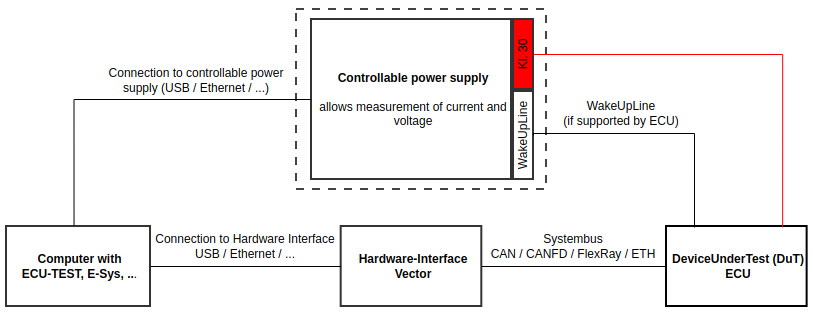
\includegraphics[width=1\textwidth]{figures/Hardware_setup.PNG}
  \caption{Sketch of a traditional test setup with an actual ECU.} \label{fig:hardware_test_setup}
\end{figure}

\begin{figure}[htpb]
  \centering
  \rotatebox{0}{ % Rotate the image by 90 degrees
    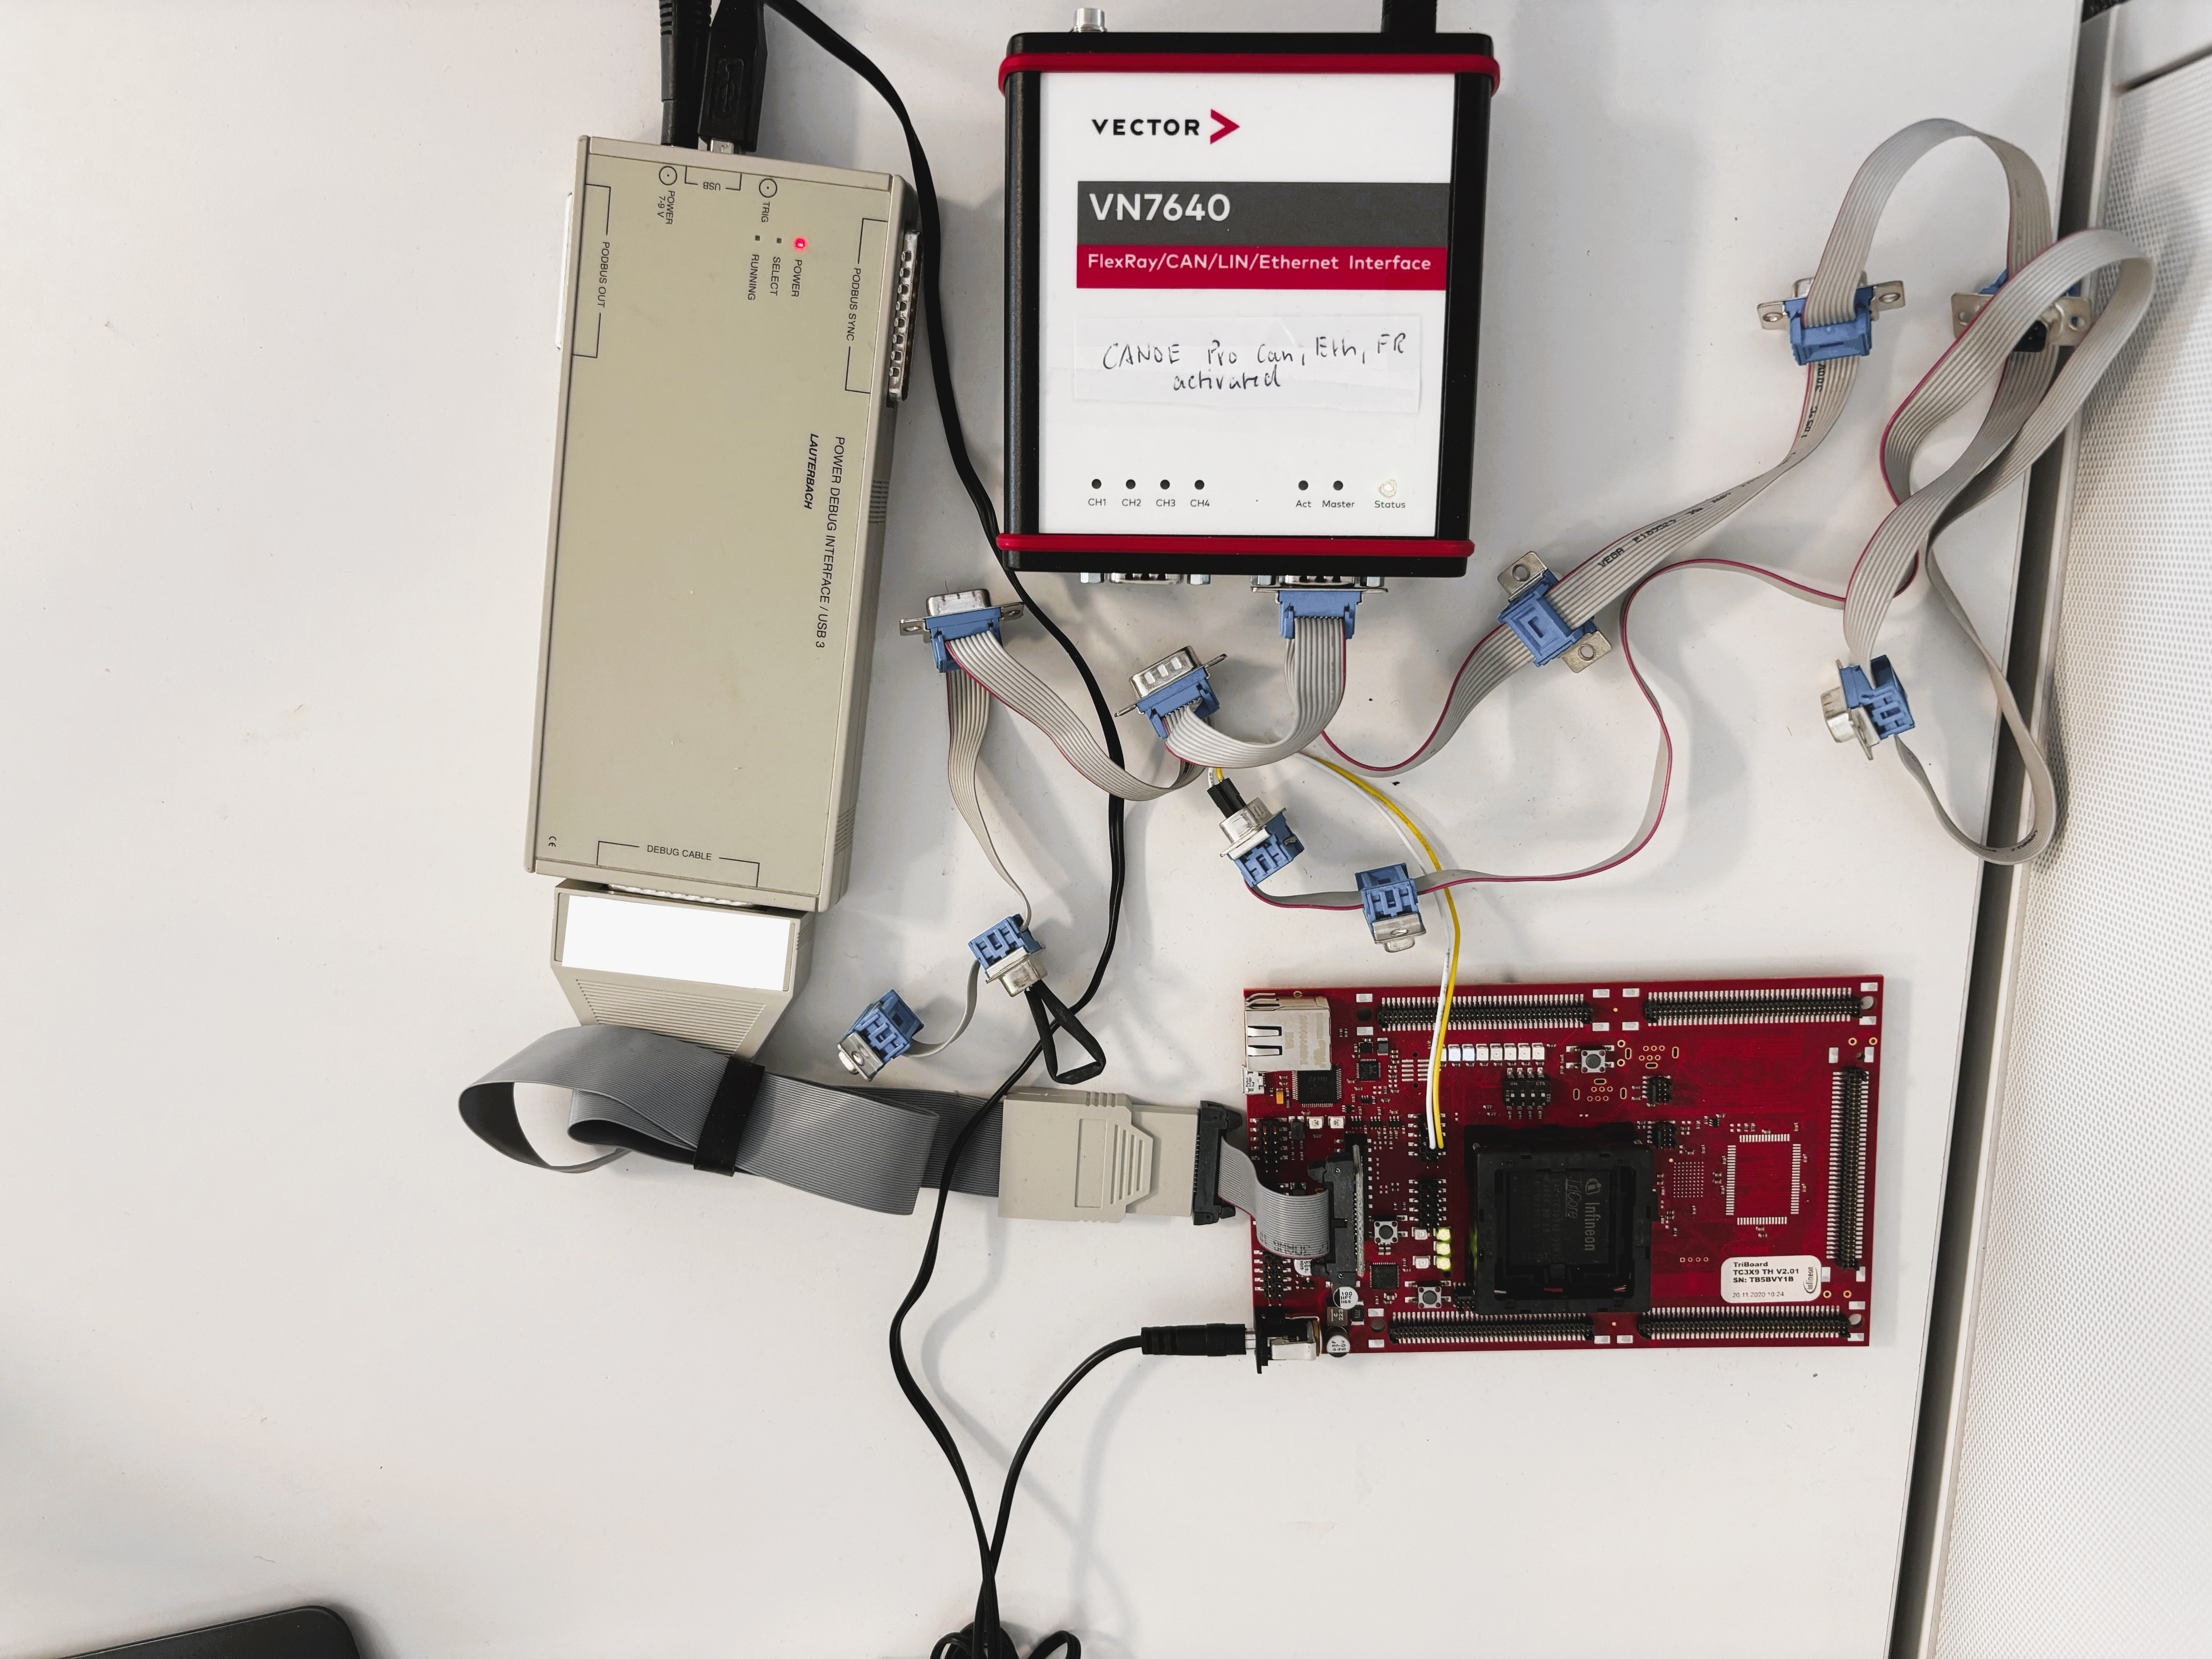
\includegraphics[width=0.65\textwidth]{figures/Real_hardware.jpg}
  }
  \caption{Real image of an ECU test setup.} 
  \label{fig:Real_hardware}
\end{figure}





\section{The Virtual Test Setup}
The objective of the virtual test setup is to replicate the functionality of the traditional hardware setup without the need for physical hardware. To achieve this, the real CAN bus is replaced with a virtual CAN bus (vCAN), as the test tools are already compatible with this interface. Next, the Vector hardware interface is substituted with "SIL KIT", which is a software capable of integrating the virtual ECU (vECU) into the simulation environment. Additionally, an adapter is required to facilitate the transmission of CAN messages between the vCAN and the vECU. \autoref{fig:test_setup} depicts the fully virtualized test setup implemented to replace the traditional hardware configuration. A detailed explanation and description of this implementation will be provided in the subsequent chapters.


\begin{figure}[htpb]
  \centering
  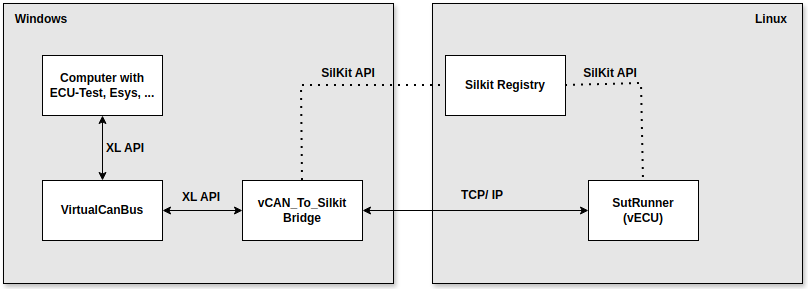
\includegraphics[width=0.97\textwidth]{figures/test_setup2.PNG}
  \caption{vECU test setup.} \label{fig:test_setup}
\end{figure}


\section{Simulation Host Environment}
As depicted in \autoref{fig:test_setup}, the testing simulation environment is divided between Linux and Windows platforms. This split is due to the current development and testing infrastructure. All BAC software development primarily takes place on Linux, and the Continuous Integration (CI) systems are also predominantly Linux-based. Running tests and executing processes on Linux is more efficient, largely due to the advantages Linux offers, such as containerization, which simplifies the CI workflow.





On the other hand, tools like ECU-Test and Esys are traditionally Windows-based. While there is a Linux version of Esys, it is limited to command-line functionality. Although the long-term plan is to move entirely to Linux, for now, Windows is still required for certain aspects of the testing process.

While it is technically possible to run the entire SIL Kit simulation on Windows and compile the source code there, this approach doesn't align with the broader strategy of maintaining a Linux-centric development and testing environment. The emphasis on containerization in the CI pipeline—especially in environments like AWS and on BMW’s servers—makes Linux the preferred choice, as Windows lacks the robust container support that Linux provides.

\section{vVIRTUALtarget}
vVIRTUALtarget is an innovative tool that allows for the simulation and testing of ECU software without needing real target hardware. It achieves this by providing virtualized OS and MCAL (Microcontroller Abstraction Layer) modules, which are essential for running the virtual ECUs generated by vVIRTUALtarget in custom environments. The virtualization technique used is very similar to that discussed in \autoref{sec:RTOS} for RTOS virtualization. ~\autoref{fig:vVirtualTarget} shows where the vVIRTUALtarget modules are located in the AUTOSAR architecture. \cite{vector_vvirtualtarget}

\begin{figure}[htpb]
  \centering
  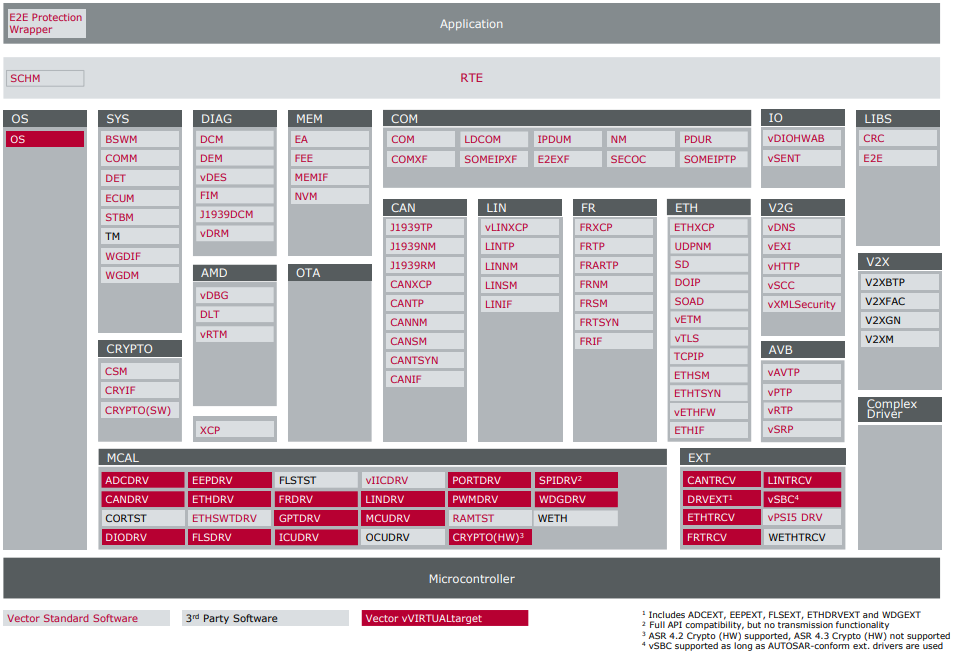
\includegraphics[width=0.83\textwidth]{figures/vVirtualTarget.PNG}
  \caption{vVIRTUALtarget virtualized layers In The 
AUTOSAR architecture \cite{user_man}.} \label{fig:vVirtualTarget}
\end{figure}

The tool is versatile, supporting various build systems, compilers, and development environments, including CMake, Microsoft Visual Studio, and MinGW-w64. Essentially, the virtual ECU generated by vVIRTUALtarget is a Windows Dynamic Link Library (DLL) or a Linux shared object (.so) file, which can be integrated with other testing tools using the OpenSUT programming interface.

The process of generating a virtual ECU involves using DaVinci Configurator Classic to configure, validate, and generate the basic software (BSW) and runtime environment (RTE) of an AUTOSAR Classic ECU. Once the project is validated and the code is generated, the project file (.vttproj) can be opened in vVIRTUALtarget. The tool then generates a Microsoft Visual Studio solution for windows or a Cmake file for linux, to create a DLL/SO for the virtual ECU.

Key configuration steps include defining application source files to be included in the solution. The tool automatically generates several files, such as:
\begin{enumerate}
\item \textbf{CANoeEmu\_cfg.c: } A source file containing handler functions for the runtime library.
\item \textbf{Vtt\_Hook.c and Vtt\_Hook.h: }Provide hook and handler functions for vVIRTUALtarget.
\end{enumerate}

vVIRTUALtarget not only generates a virtual ECU but also creates a standalone System Under Test (SUT) executable, enabling out-of-the-box connectivity with the Vector SIL Kit. When running as a standalone SUT, the virtual ECU operates as a separate process and can interact with tools like CANoe via the Vector SIL Kit, leveraging the OpenSUT API for flexible integration into a custom environment. \cite{user_man}

\subsection{Structure of the Shared Object Simulation}\label{subsec:structure_of_simulation}
Within the shared object, there is a directory named "\textbf{CanoeEmu}", which houses both header and source files essential for the simulation process. This directory includes key files such as "\textbf{CANoeEmuLibExport.h}", which is responsible for exporting functions from the "\textbf{libcanoe}" library, and "\textbf{CANoeEmu\_DllMain.cpp}", which provides the necessary functions to be exported from the VTT SUT Library. Additionally, "\textbf{CANoeApi.h}" contains prototypes for the CANoe APIs used throughout the simulation.

During the build process, the "\textbf{CanoeEmu}" directory is linked with the "\textbf{libcanoe}" library within the \textbf{CMake} configuration, ensuring that all required dependencies are in place. When the SUTRunner executable loads the shared object, several functions from the "\textbf{CanoeEmu}" directory are dynamically loaded and invoked at runtime. These functions play a critical role in initializing data, locating the main function within the shared object, and simulating various hardware behaviors.

The first function called upon loading the shared object is "\textbf{opensut\_init}", which is responsible for initializing the SUT. This function, in turn, calls an essential function named "\textbf{CANoeAPI\_InitHook}". The "\textbf{CANoeAPI\_InitHook}" must be implemented by any application utilizing the CANoe emulation library, as it serves as the central initialization hook for the emulation. Within this initialization hook, various init functions can be used to configure multiple aspects of the emulation, ensuring that the system is properly set up for accurate simulation.

\section{Vector SIL Kit}
Vector SIL Kit (Software-in-the-Loop Kit) is a versatile tool designed for simulating, testing, and validating distributed automotive systems, particularly focusing on environments with virtual ECUs. SIL Kit enables co-simulation, allowing multiple ECUs and other system components to interact within a unified simulation environment. This removes the need for physical hardware during testing, making it especially useful in early development stages. SIL Kit supports complex automotive testing scenarios, including system interactions, timing, and performance analysis, using simulated networks such as CAN or Ethernet, replicating the communication in real vehicle systems. \cite{sil_kit_github}

\subsection{How SIL Kit Works}
A SIL Kit simulation setup consists of several key components: the \textbf{SIL Kit Registry} and one or more simulation \textbf{participants} (e.g., virtual ECUs). The \textbf{SIL Kit Registry} plays a central role, as it is responsible for connecting and managing communication between all participants. The registry must be started before any participants are created, acting as a broker that enables discovery and connection between participants.

Here’s a breakdown of the SIL Kit process \cite{sil_kit_docs}:

\begin{enumerate}
\item \textbf{Registry: } The SIL Kit Registry is the first component that must be launched. It listens for participants on a specified URI and provides connection information, allowing participants to establish peer-to-peer connections.
\item \textbf{Participants: } Each participant, whether it's a virtual ECU or another software component, connects to the registry to obtain information about other active participants. Once the connection information is exchanged, participants communicate directly, forming a simulation network. SIL Kit supports network types like TCP/IP and Unix Domain Sockets to facilitate these connections.
\item \textbf{Simulation Setup: } When a new participant joins, it opens a public listening socket and connects to the registry. The registry then provides the participant with the connection details of other participants, enabling direct peer-to-peer communication. By default, participants attempt to connect via Unix Domain Sockets and fall back on TCP if necessary.
\item \textbf{Simulation Task: } The actual simulation happens through a callback mechanism, which is triggered as simulation time progresses. This is done using the time synchronization service by registering the \textbf{SetSimulationStepHandler()} callback. 
\end{enumerate}

\begin{figure}[htpb]
  \centering
  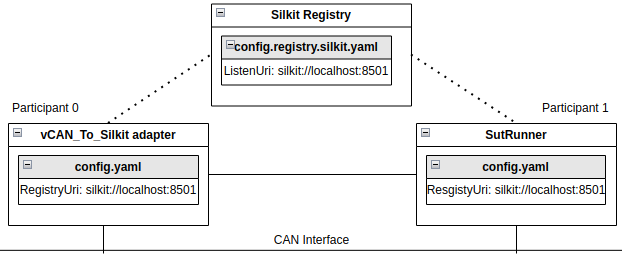
\includegraphics[width=0.83\textwidth]{figures/silkit_connection.PNG}
  \caption{ Simulation setup with two participants that communicate on a CAN bus network.} \label{fig:silkit_conn}
\end{figure}

\subsection{Integration with vVIRTUALtarget}
In this project, SIL Kit integrates seamlessly with vVIRTUALtarget. The SutRunner generated by vVIRTUALtarget is connected to the SIL Kit environment as a participant in the simulation. Additionally, an adapter is developed and connected to SIL Kit as a separate participant.

As shown in \autoref{fig:silkit_conn}, the two participants— the SutRunner and the adapter— exchange their connection information through the SIL Kit Registry, enabling smooth communication over a simulated network. This setup ensures that the vECU and the testing tools can interact within a cohesive simulation, mimicking real-world conditions for early testing and debugging.

\subsection{Time Synchronization in SIL Kit}
When the \textbf{TimeSyncService} is used in SIL Kit, participants follow a synchronized virtual time framework, ensuring that each component in the distributed simulation advances in lockstep with the others. The service allows for configuring the size of each simulation step and setting up handlers that get called at each step. As the virtual time progresses, the step handler is triggered to allow the participant to carry out its tasks at that moment. SIL Kit guarantees that the virtual time moves forward consistently—without skipping or repeating any steps—according to the configured interval for each participant. \cite{sil_kit_docs}

\subsubsection{Autonomous vs. Coordinated Modes}
SIL Kit offers two modes of operation for participants: \textbf{Autonomous} and \textbf{Coordinated}. When running in \textbf{Coordinated} mode, participants synchronize their states, ensuring that all essential components are aligned before beginning the simulation. This coordinated setup is necessary when multiple participants need to reach the Running state simultaneously, as the simulation will only start once all participants are ready. If one participant calls Stop(), the entire group of coordinated participants will pause, making this mode suitable for tightly synchronized environments where collective actions are essential.

On the other hand, in \textbf{Autonomous} mode, each participant runs independently of the others. In this mode, participants don’t wait for synchronization, and each can start and stop its simulation without affecting the others. This is ideal for situations where timing synchronization is unnecessary across participants, allowing for more flexibility.

\subsubsection{Synchronization Between the vECU and the Adapter}
In this project, \textbf{vVIRTUALtarget} originally used Coordinated mode for the \textbf{SutRunner}, expecting the vECU to synchronize with other virtual ECUs in the system. However, since the \textbf{ECU-Test} tool operates in real time, it wouldn’t make sense to coordinate the adapter with the virtual time, as the adapter’s role is simply to forward CAN messages as they arrive. Coordinating the adapter would only make sense if ECU-Test was also working with virtual time, which it isn’t.

Because of this, the \textbf{SutRunner} was switched to \textbf{Autonomous mode}, allowing it to function independently. In this setup, the adapter forwards messages in real time, and the simulation doesn’t require strict synchronization with the vECU. This adjustment ensures that the real-time nature of ECU-Test is maintained, while still leveraging the benefits of the virtual environment.

\section{Vector XL Library}
The Vector XL Library is another essential tool that will be utilized in this project. It provides a comprehensive set of functions and APIs for interacting with Vector's hardware and software products, facilitating communication and data exchange within automotive networks.

The XL Library abstracts the complexities of hardware communication, allowing developers to interact with various bus systems such as CAN, LIN, FlexRay, and Ethernet using a consistent API. This abstraction simplifies the development process and ensures compatibility across different hardware setups.

The Vector Hardware Config tool is required to set up the hardware settings like virtual channel assignment etc. The management of the application settings can be either done in the tool or via get/set functions of the XL Driver Library. \cite{xl_driver_library_manual}

\section{Software tools for testing}
In the context of BMW vehicles, there are multiple software tools used for testing and validating the ECUs, such as AmTS and Esys.

The development, testing, and validation of vehicle software and hardware components, including Electronic Control Units (ECUs), within BMW vehicles are facilitated by a comprehensive quality assurance technology stack known as the Automotive Test Suite (AmTS) \cite{automotive_test_suite_2022}. This system serves as the foundation for a streamlined and automated testing process, where relevant test plans are implemented in the "\textbf{ECU-TEST}" automation tool and executed automatically for each ECU. The test results are then seamlessly integrated into the "\textbf{TEST-GUIDE}" test report management system, providing clear and accessible data for all stakeholders involved.

\textbf{Esys} is another specialized software tool that is widely utilized by BMW engineers to code, program, and configure the ECUs in BMW vehicles. This software tool plays a vital role in the overall process of ensuring the proper functioning and integration of the vehicle's electronic systems.


\section{Unified Diagnostic Services (UDS)}
The Unified Diagnostic Services (UDS) protocol is a key communication system used in automotive diagnostics \cite{iso_14229}. It enables diagnostic tools to interact with an ECU by sending requests and receiving responses, much like how diagnostic communication works on physical cars. The UDS protocol can be understood as a communication method between a testing tool and the ECU in vehicles, somewhat analogous to HTTP requests used on the web. Both UDS and HTTP requests follow a request-response model, but they operate in different contexts.

UDS operates on the CAN bus and is used for various tasks such as fault diagnosis, reading sensor data, and flashing firmware. Through standardized services, UDS allows for complex operations such as software updates, troubleshooting, and testing the behavior of ECUs by sending specific commands. These commands use service identifiers (SIDs), like the commonly used 0x22 for "Read Data by Identifier" to extract system data\cite{uds_tutorial}.

In the context of testing virtual ECUs (vECUs), UDS messages are essential because they simulate the same interactions a real-world ECU would encounter. By sending UDS requests over a virtual CAN (vCAN) bus, we can validate whether the vECU behaves as expected, ensuring it is capable of handling real-world diagnostic operations. This process is crucial during testing phases to ensure the system's accuracy before physical deployment.\\


In conclusion, the combination of vVIRTUALtarget, Vector SIL Kit, and the Vector XL Library forms a comprehensive ecosystem for the simulation, testing, and validation of virtual ECUs. These tools enable the development of sophisticated and reliable automotive software, allowing for thorough testing in both virtual and hybrid environments. However, some adaptations are still needed to achieve a fully virtual test setup.